% Author: Izaak Neutelings (June 2017)
% taken from https://tex.stackexchange.com/questions/53445/how-to-draw-spherical-geometries-with-tex

\documentclass[border=1pt,tikz]{standalone}
\usepackage{amsmath}
\usepackage{enumerate}
\usepackage{tikz}
\usepackage{xcolor}
\usepackage{tikz-3dplot}
\usepackage{hyperref}
\usepackage{pgfplots}
\usetikzlibrary{calc,3d,intersections,positioning,shapes,patterns,pgfplots.fillbetween}
\pgfplotsset{compat=1.11} 



\newcommand{\InterSec}[3]{%
  \path[name intersections={of=#1 and #2, by=#3, sort by=#1,total=\t}]
  \pgfextra{\xdef\InterNb{\t}}; }

\begin{document}



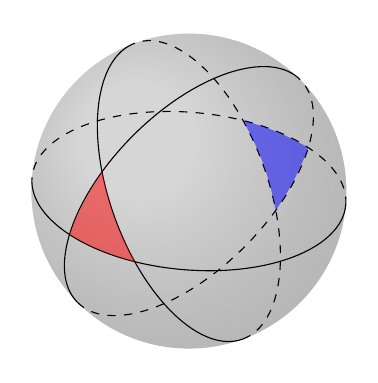
\begin{tikzpicture}

  \pgfmathsetmacro\R{2} 
  \fill[ball color=white!10, opacity=0.2] (0,0,0) circle (\R); % 3D lighting effect
  
  \foreach \angle[count=\n from 1] in {-5,225,290}{
    \begin{scope}[rotate=\angle]
      \path[draw,dashed,name path global=d\n] (2,0) arc
           [start angle=0,end angle=180,x radius=2cm,y radius=1cm];
      \path[draw,name path global=s\n] (-2,0) arc
           [start angle=180,end angle=360,x radius=2cm,y radius=1cm];
    \end{scope}
  }
  
  \InterSec{s1}{s2}{I3};
  \InterSec{s1}{s3}{I2};
  \InterSec{s3}{s2}{I1};
  \fill[fill=red,opacity=0.5] (I1) to [bend right=8.5]  (I2) to [bend left=7] 
  (I3) to [bend left=6] (I1);
  
  \InterSec{d1}{d2}{J3};
  \InterSec{d1}{d3}{J2};
  \InterSec{d3}{d2}{J1};
  %\fill[blue] (J1)--(J2)--(J3)--cycle;
  
  \fill[fill=blue,opacity=0.5] (J1) to [bend right=8.5]  (J2) to [bend left=7] 
  (J3) to [bend left=6] (J1);

\end{tikzpicture}



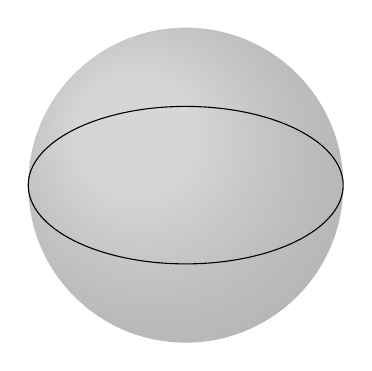
\begin{tikzpicture}

  \pgfmathsetmacro\R{2} 
  \fill[ball color=white!10, opacity=0.2] (0,0,0) circle (\R); % 3D lighting effect

  \path[draw,name path global=d1] (2,0) arc [start angle=0,end angle=360,
        x radius=2cm,
        y radius=1cm];
  
%  \foreach \angle[count=\n from 1] in {-5,225,290}{
%    \begin{scope}[rotate=\angle]
%      \path[draw,dashed,name path global=d\n] (2,0) arc [start angle=0,
%        end angle=180,
%        x radius=2cm,
%      y radius=1cm];
%      \path[draw,name path global=s\n] (-2,0) arc [start angle=180,
%        end angle=360,
%        x radius=2cm,
%      y radius=1cm];
%    \end{scope}
%  }
  
%  \InterSec{s1}{s2}{I3};
%  \InterSec{s1}{s3}{I2};
%  \InterSec{s3}{s2}{I1};
%  \fill[fill=red,opacity=0.5] (I1) to [bend right=8.5]  (I2) to [bend left=7] 
%  (I3) to [bend left=6] (I1);
%  
%  \InterSec{d1}{d2}{J3};
%  \InterSec{d1}{d3}{J2};
%  \InterSec{d3}{d2}{J1};
%  \fill[fill=blue,opacity=0.5] (J1) to [bend right=8.5]  (J2) to [bend left=7] 
%  (J3) to [bend left=6] (J1);

\end{tikzpicture}



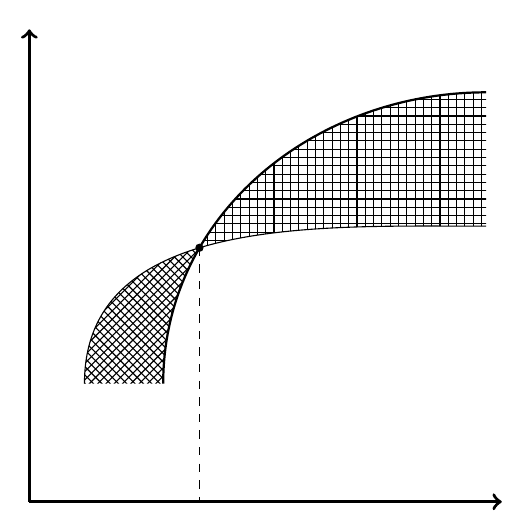
\begin{tikzpicture}

  \draw[thick,name path=thick] 
    (1.7, 1.5) to[out=90,in=180] (5.8, 5.2);
  \draw[name path=thin] 
    (.7, 1.5) to[out=90,in=180] (5.8, 3.5) ;
  \draw[->, very thick] (0,0) -- (6,0);
  \draw[->, very thick] (0,0) -- (0,6);
  \fill[name intersections={of=thick and thin, by={intersect}}] 
    (intersect) circle (1.5pt);
  \draw[dashed] (intersect) -- (intersect |- 0,0);
  \tikzfillbetween[
    of=thick and thin,split,
    every even segment/.style={pattern=crosshatch}
  ] {pattern=grid};
  
\end{tikzpicture}



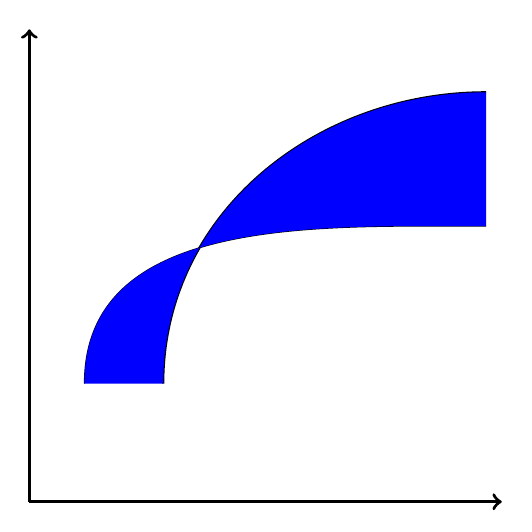
\begin{tikzpicture}

  \draw[thick,name path=thick] 
    (1.7, 1.5) to[out=90,in=180] (5.8, 5.2);
  \draw[name path=thin] 
    (.7, 1.5) to[out=90,in=180] (5.8, 3.5) ;
  \draw[->, very thick] (0,0) -- (6,0);
  \draw[->, very thick] (0,0) -- (0,6);
  \tikzfillbetween[
    of=thick and thin
  ] {blue};
  
\end{tikzpicture}



\usetikzlibrary{shapes.geometric}
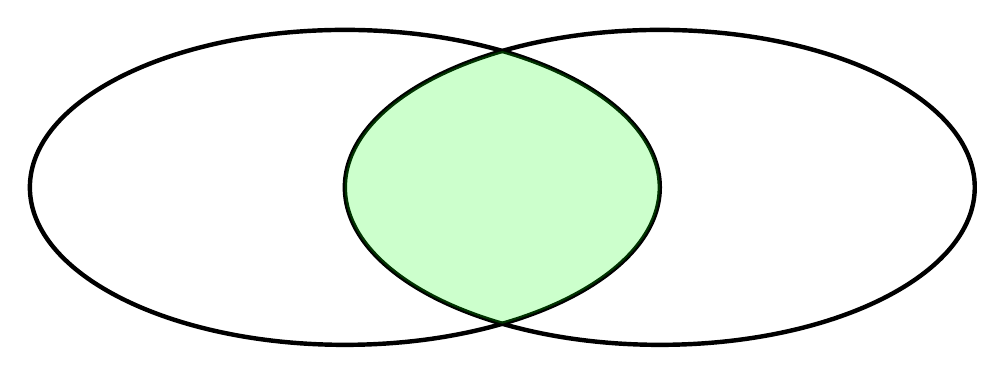
\begin{tikzpicture}
  \def\R{2cm}
  \def\A{(0,0) ellipse [x radius=2*\R,y radius=\R]}
  \def\B{(4,0) ellipse [x radius=2*\R,y radius=\R]}
  \node[draw, shape=ellipse, minimum width={4*\R}, minimum height={2*\R}, ultra thick]
    (A) at (0,0) {};
  \node[draw, shape=ellipse, minimum width={4*\R}, minimum height={2*\R}, ultra thick]
    (B) at (4,0) {};
  \begin{scope}
    \clip \A;
    \fill[green, opacity=0.2] \B;
  \end{scope}
\end{tikzpicture}



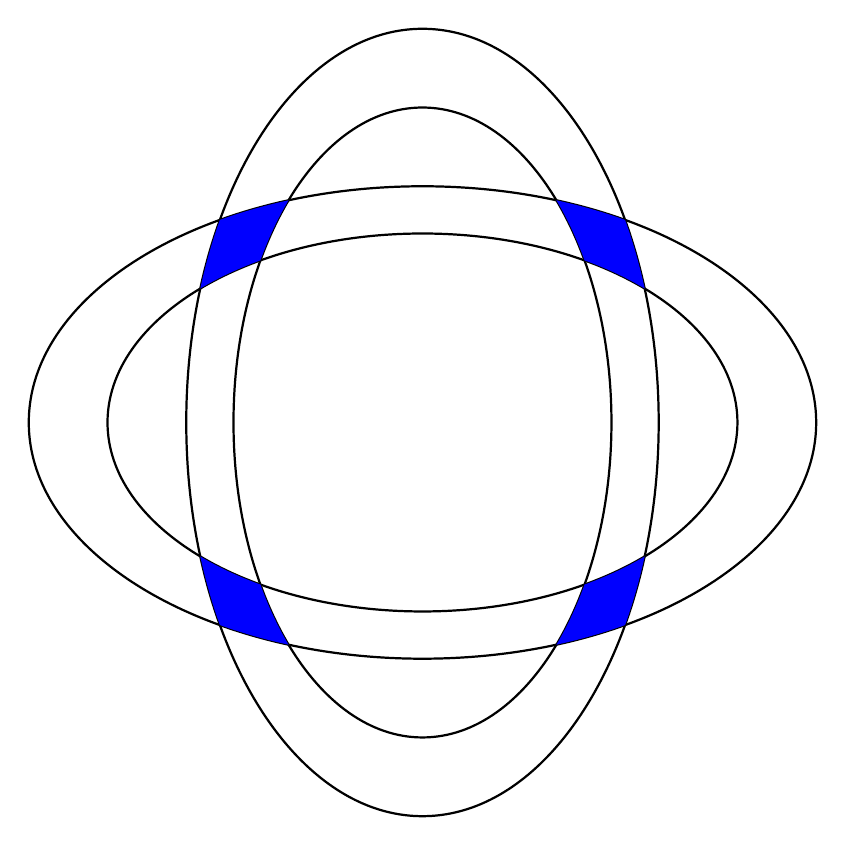
\begin{tikzpicture}
  \def\R{5}
  \def\Rx{3}
  \def\b{0.8}
  \def\Xa{(0,0) ellipse ({   \R } and {   \Rx})}
  \def\Xb{(0,0) ellipse ({\b*\R } and {\b*\Rx})}
  \def\Ya{(0,0) ellipse ({   \Rx} and {   \R })}
  \def\Yb{(0,0) ellipse ({\b*\Rx} and {\b*\R })}
  \def\Sa{(-\R,-\R) rectangle (\R,\R)}
  \def\Sb{(  0,  0) rectangle (\R,\R)}
  
  \draw[thick] \Xa;
  \draw[thick] \Xb;
  \draw[thick] \Ya;
  \draw[thick] \Yb;
  
  \begin{scope}
    \clip \Xa;                    % clip away everything outside \Xa
    \clip[insert path={\Sa}] \Xb; % clip away everything inside  \Xb
    \clip[insert path={\Sa}] \Yb; % clip away everything inside  \Yb
    %\clip \Sb;                   % only select right upper quadrant
    \fill[blue] \Ya ;
  \end{scope}
  
\end{tikzpicture}



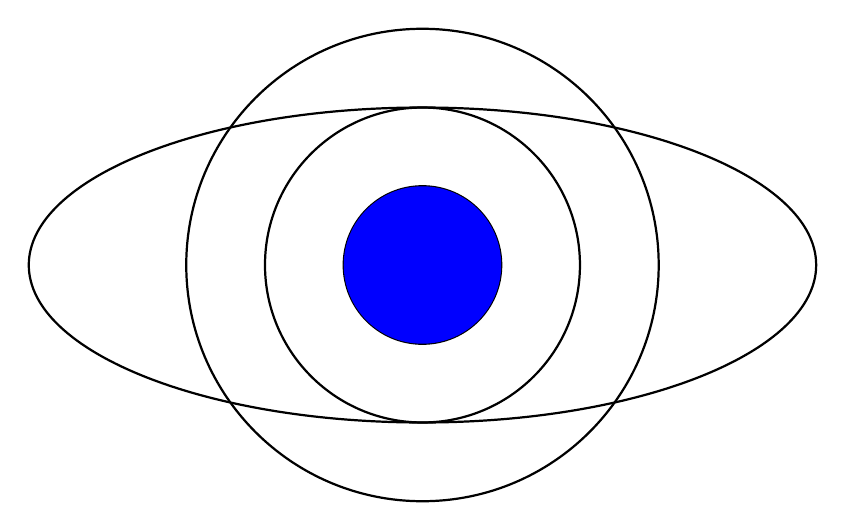
\begin{tikzpicture}
  \def\R{1}
  \def\A{(0,0) ellipse ({  \R} and {  \R})}
  \def\B{(0,0) ellipse ({2*\R} and {2*\R})}
  \def\C{(0,0) ellipse ({3*\R} and {3*\R})}
  \def\E{(0,0) ellipse ({5*\R} and {2*\R})}
  
  \draw[thick] \A;
  \draw[thick] \B;
  \draw[thick] \C;
  \draw[thick] \E;
  
  \begin{scope}
    \clip \C;
    \clip \A;
    \fill[blue] \B ;
  \end{scope}
  
\end{tikzpicture}



\end{document}